\documentclass[a4paper, onecolumn, 12pt]{article}
\usepackage[left=33mm,right=33mm,top=35mm,columnsep=15pt]{geometry} 

% basic packages
\usepackage[english]{babel} %language
\usepackage[utf8]{inputenc} %input encoding
\usepackage{float} %position of floating objects
\usepackage{bookmark} %hyperlinks in pdf
\usepackage{subcaption}
\usepackage[T1]{fontenc}
\usepackage{lipsum} %placeholder text

% math packages
\usepackage{amsthm} %theorems
\usepackage{amsmath} %math
\usepackage{mathtools} %still math

% code packages
\usepackage{listings} %code
\usepackage{xcolor} %syntax highlighting
\usepackage{algorithm}
\usepackage{algpseudocode}
\usepackage{fancyvrb}

% todonotes package
\usepackage{xkeyval}
\usepackage{tikz}
\usepackage{calc}
\setlength {\marginparwidth }{2cm}
\usepackage{todonotes} % Load the todonotes package

% custom commands
\newcommand\tab[1][.3cm]{\hspace*{#1}}
\newcommand\tabeq[1][.5cm]{\hspace*{#1}}
\newcommand\suggestion[1]{\textcolor{violet}{\textbf{Suggestion}: #1}}
\newcommand\old[1]{\textcolor{brown}{\textbf{Old}: #1}}
\newcommand\doubt[1]{\textcolor{purple}{#1 \textbf{(?)}}}
\newcommand\code[1]{\textcolor{teal}{\texttt{#1}}}

% \usepackage{physics}
% \usepackage{adjustbox}
% \usepackage{placeins}
% \usepackage{csquotes}
% \usepackage[normalem]{ulem}
% \useunder{\uline}{\ul}{}

\title{Interaction with a Nao Humanoid robot in competitive games \\ Elective in AI / HRI Report}
\author{Flavio Maiorana \and Valerio Spagnoli \and Flavio Volpi}
\date{\today}

\begin{document}

\maketitle

\section{Introduction}
\label{sec:intro}
In the RoboCup games, robots are fully autonomous, yet there is potential for 
improvement through human interaction. Just as human soccer players benefit from 
receiving real-time suggestions or explicit instructions during a match, 
autonomous soccer robots could also enhance their performance by incorporating 
informed guidance. 
In this project, we aim to take a step in this direction by developing a 
system that enables a human operator to interact with a Nao humanoid robot via a graphical 
interface and voice commands. The goal is to enhance the robot's performance and 
provide real-time strategic suggestions, similar to the role of a football coach.

\subsection{Context and Motivation}
\label{sec:context}

\subsubsection{RoboCup SPL Challenge}
This project was specifically designed to be used in the RoboCup 2024 SPL challenge, 
where two robots of one team had to compete against two robots of the opponent team, 
and one of the two robots for each team was controlled by a human operator. Furthermore, 
the rules of the challenge forced the human operator to turn his back to the field, 
in order to not directly observe the environment. This constrained us to make use of the
directional robot-human communication also for the reconstruction of the world model.

\subsubsection{Possible Extensions}  
The system developed in this project could be adapted to various other contexts. For instance, 
it could be applied to the RoboCup SPL main competition, where a human operator for each team 
might be allowed to provide real-time instructions to the robots via voice commands, using the 
graphical interface to view the reconstructed world model of the entire team.  

Another potential extension involves modifying the system to enable robots to play alongside human players. 
In this scenario, the robot would need to interpret human commands and execute them in real-time, allowing 
for mixed teams of humans and robots in a soccer game.

\subsection{Objectives}
\label{sec:obj}

In the context of the RoboCup SPL challenge, the main objective of the project is to develop a framework
that allows the human operator to use the robot as a \textit{proxy} to interact with the environment, namely the soccer
field. 
To do this, a form of bidirectional interaction between the human operator and the controlled robot is necessary. 

\subsubsection{Bidirectional Communication}  
Receiving instructions from a coach can significantly impact the outcome of a soccer match. 
Likewise, getting feedbacks from the robot when issuing commands greatly enhances 
the quality of the interaction. The human, acting as a coach, must be completely aware of the robot's surroundings,
while the robot must be able to interpret the human's commands and respond accordingly. 
\begin{itemize}  
    \item \textbf{Robot-to-Human Communication}: The robot provides the human operator with 
    all the necessary information to reconstruct the world model. These data are transmitted 
    over the network to the operator's computer, where are filtered and displayed on the 
    graphical interface. Moreover, the robot responds with vocal feedbacks to the confirm received 
    commands or to report any issues (e.g. the impossibility to execute the command).  
    \item \textbf{Human-to-Robot Communication}:  
    \begin{itemize}  
        \item \textbf{Coach-to-Robot Communication}: The human operator, acting as a coach, can 
        analyze the reconstructed world model using the graphical interface and decide to send commands to the robot. 
        The latter are transmitted through the network or via voice commands.  
        \item \textbf{Referee-to-Robot Communication}: In the context of the RoboCup 
        SPL challenge, another human, acting as a referee, can send commands to the robot using 
        whistle signals. The robot must be capable of interpreting these signals and responding 
        accordingly.
    \end{itemize}  
\end{itemize}

\begin{figure}
    \centering
    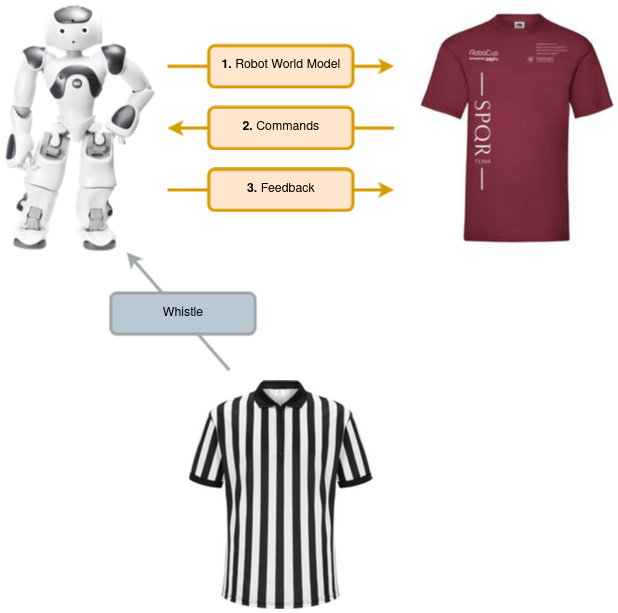
\includegraphics[width=0.7\linewidth]{assets/bidirectional-communication.png}
    \label{fig:bidirectional-communication}
    \caption{Bidirectional communication scheme}
\end{figure}


\subsubsection{Real-time Interaction}
In the context of the RoboCup SPL challenge, the system must process commands in real-time, given the 
competitive nature of the scenario. The robot needs to promptly interpret and execute the human operator's 
commands while providing immediate feedback on the execution status. Any delay in processing could adversely 
affect the robot's performance and the outcome of the match. Even in other applications, real-time interaction 
is critical to maintain the robot's responsiveness to human input and ensure accurate reconstruction of the robot's world model.

\subsection{Summary of the results}
\label{sec:summary}

Our system achieved the goal of allowing a human operator to control a Nao
by voice and using a graphical interface, and to receive feedbacks from the robot
in response to the commands. The system integrates various features, such as:
\todo[inline]{forse dire che il mental model del robot già esiste???}
\begin{itemize}
    \item \textbf{communication}: which manages the communication between the robot and
    the human operator
    \item \textbf{mental model}: responsible for representing the field by
    accessing only the robot's perceptions
    \item \textbf{interaction}: by answering to the commands before executing
    them, considering also the feasibility of the execution itself,
    \item \textbf{memory}: the robot has a memory of some information about the 
    environment, and about some events happened in the past.
    \suggestion{the past command is held in memory, in order to
    resume it in case it is needed}.
\end{itemize}
The system was tested in the RoboCup 2024 SPL challenge, where SPQR Team reached
the third place, demonstrating the effectiveness of the system in a competitive
environment.

\newpage

\section{Related Work}
\label{sec:rel}

Interpreting human signals has been a challenge for some time now in Robotics.
Humans communicate through various modalities, including vision, audio, and
motion. This multimodal nature provides rich information that sensory inputs can
capture and analyze. 

Recent advances in Deep Learning have facilitated the
integration of multimodal data, significantly improving the comprehension of
relationships within individual modalities, a key factor for precise message
interpretation \cite{LIU20183} \cite{su2023recent}.

In RoboCup Soccer, human-robot interaction is predominantly one-way, with human
referees conveying game states and events to robots. A significant trend in the
RoboCup SPL is the progressive reduction of network communication in
favor of human-like signal interpretation, allowing robots to interpret human
signals more naturally. \cite{digiambattista}

A notable case worth to mention is also \cite{antonioni}, where they propose an
approach to improve the decision making process through the audience noise by
extracting relevant features through MFCC coefficients and applying a
reinforcement learning pipeline. 

This case could fall into a broader category where the goal is to improve the
communication from an ideal coach to the robot in order to improve planning and
decision-making. In particular, \cite{musumeci} tackles this problem by
designing a system that enriches the planning process with temporal goals and
constraints given by human indications. 

Our work is inspired by these studies, and the goal is to develop a system that
allows a human operator to have a one-to-one interaction with a robot, acting
like a coach in a soccer match.

\newpage
\section{Solution}
\label{sec:sol}

The system can be divided in three parts: 
    \begin{itemize}
        \item framework backbone, written in C++, which runs on the robot itself;
        \item interface in Node.js, where the reconstructed world
        model is displayed and the commands to control the robot are available; 
        \item Python server, which allows the comunication between the robot 
        and the interface, i.e. it is responsible for issuing commands to the robot 
        and receiving feedback or sensory information. 
    \end{itemize}

\subsection{Framework backbone}
\label{sec:framework}
The framework on which everything stands on is the one of the SPQR team of Sapienza University \cite{spqr},
which is derived from that one of the
German team B-Human of the year 2021 \cite{bhuman2023}, University of Bremen. At low level, the robot is 
controlled by four threads:
\begin{itemize}
    \item \textbf{Upper camera thread}: it deals with upper camera of the robot, positioned on its forehead;
    \item \textbf{Lower camera thread}: it deals with lower camera of the robot, placed on its chin;
    \item \textbf{Cognition}: it is responsible for collecting all informations from the 
    environment through cameras and sensors; also, using some informations as input,
    it returns high level commands about the actions the robot has to execute;
    \item \textbf{Motion}: it converts high level commands of the thread Cognition in effective
    motion control of the 25 joints of the robot;
\end{itemize}
Both camera threads capture images from the cameras of the robot, and work on them 
to retrieve informations to describe the world.

\begin{figure}
    \centering
    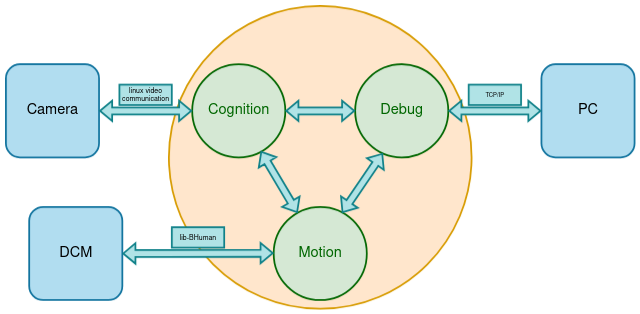
\includegraphics[width=0.5\linewidth]{assets/threads.png}
    \label{fig:threads}
    \caption{Threads}
\end{figure}

\subsubsection{Representations and Modules}
The two main components for the collection and storage of information from the environment
are called Representations and Modules.
Representations store informations at the current instant, and they represent the actual overview
of the world. Each representation is a derived class of the class $Streamable$, which allows a 
direct connection of all attributes and functions of the given representation with all other
representations and modules. Furthermore, each representation has a single module provider, which
is the only capable of modifying its attributes.

Instead, the task of the modules is to make computations which require specific inputs and returns
determined output. In details, a module can specify the representations it needs in input through
the macros REQUIRES and USES, and must specify the representations it is going to modify through
the macro PROVIDES. A module must specify a function named $update$, that has the scope to 
perform the real updates of the informations inside the provided representations.

The correct usage of REQUIRES and USES is established by a scheduler inside the software, which decides 
the right execution order of the modules according to cyclic dependencies between representations.
For example, if a module M1 updates the representation R1, and this representation is required from 
module M2 to modify its representation, the module M2 cannot be executed before the module M1, so the
scheduler will execute in order M1 and M2. 
\begin{figure}[h]
    \centering
    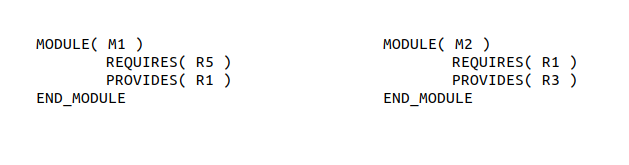
\includegraphics[width=0.8\linewidth]{assets/modules.png}
    \label{fig:modules}
    \caption{Functioning of modules and representations}
\end{figure}

Every update function has an execution frequency of 83 Hz, which practically allows an information 
refresh in real time.

\subsubsection{Behaviors and Skills\&Card}
Behaviors represent the real actions the robot will take during the game. They are modeled as finite 
automata, according to CABSL standard ($C$-$based$ $Agent$ $Behavior$ $Specification$ $Language$) \cite{CABSL}.
This is based on the concepts of options, states, transitions and actions: the options are finite-state machines that
describe a determined way of acting; transitions define the conditions to move between two states of the graph; 
when the latter arrives in a state, the specified actions are executed.
Actions are expressed as $Skills$, which are the leaves of the graph and the lowest abstraction elements.
They make calls directly to the motion engine of the robot.

Option idea matches with the concept of Card: each card represents one option, and it is the interpretation
of an higher abstraction level for the actions. 
To enter in a card, a robot has to satisfy its specified preconditions; to exit from a card, preconditions are not
satisfied anymore or its postconditions are met instead.
Cards are the fundamental elements that compose the Decks, which are literally ordered collections of cards.
The order establishes the priority of the cards: the ones on the top have higher priority than the ones on the bottom.
Starting from the first card, the agent enters in it if its preconditions are satisfied, otherwise he discards 
the card and checks the second one, and so on. So it is very important to establish the right disposition,
according to own puproses. 

This hierarchy of the system allows to link the decks to the roles of the players in the field. 
In this way it is possible to associate just the cards relative to the corresponding role, avoiding
possible undesired behaviors. 


\begin{figure}
    \centering
    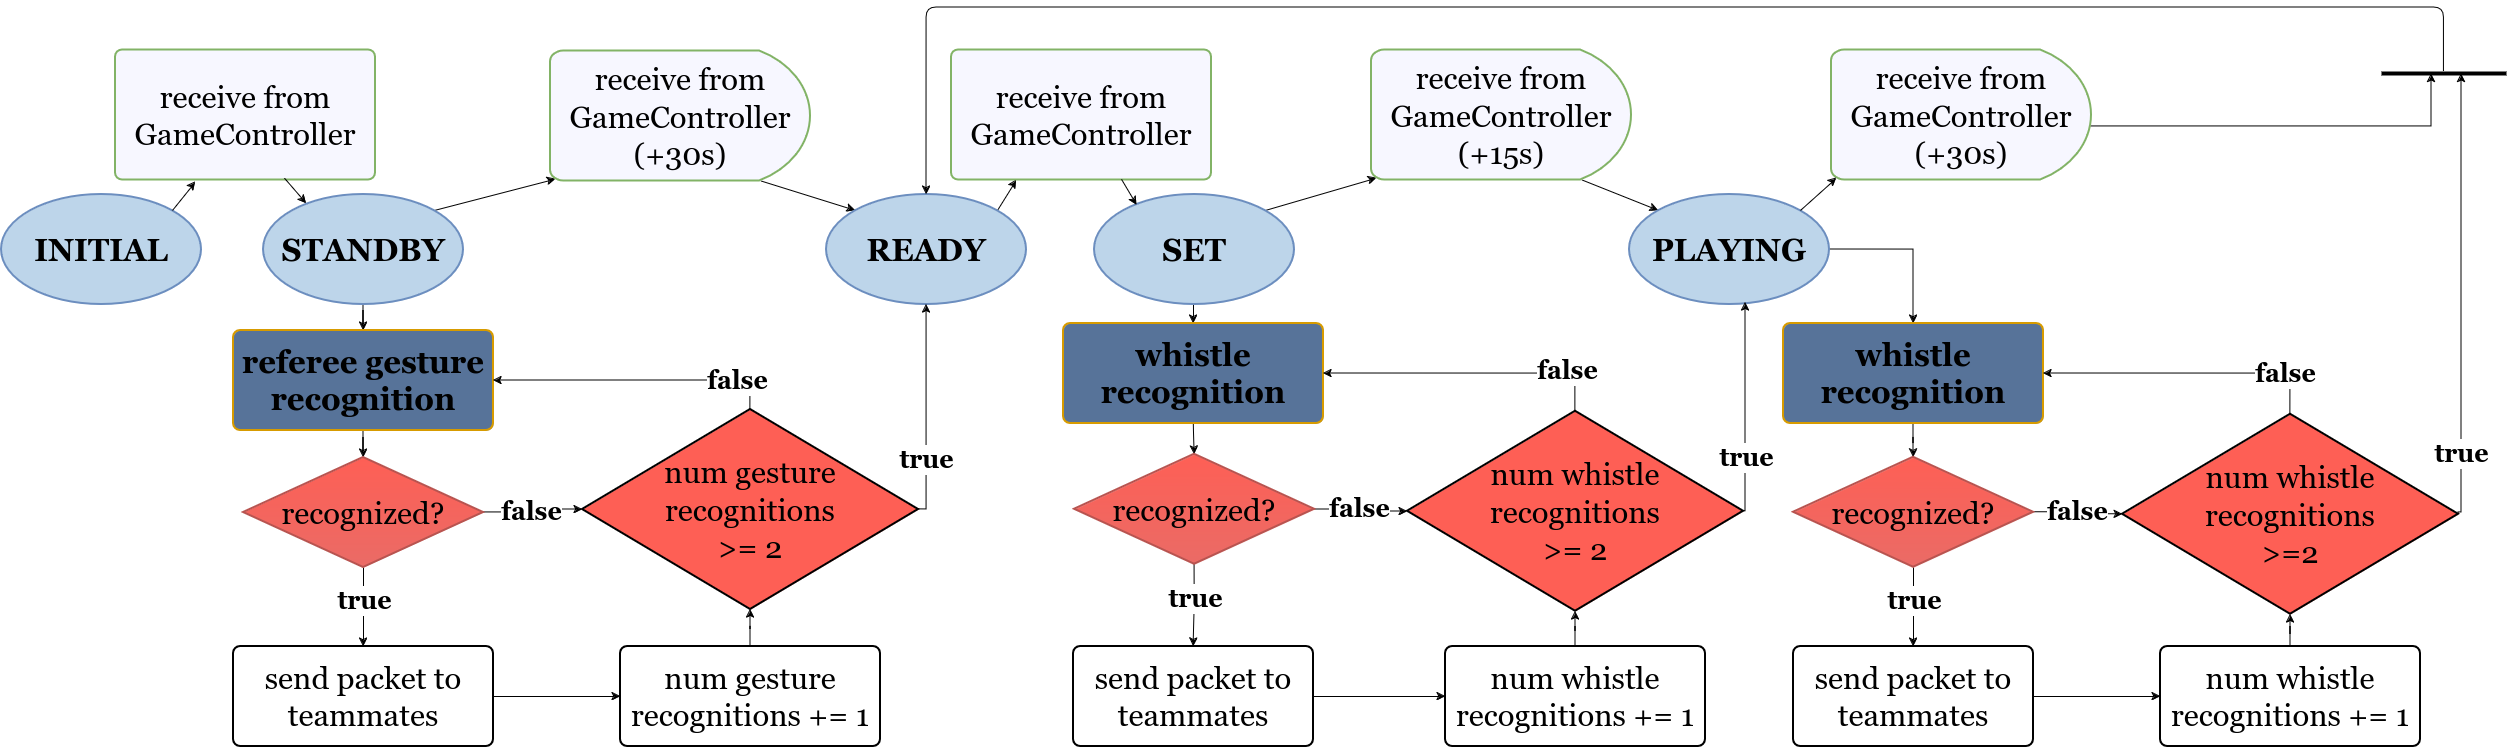
\includegraphics[width=0.9\linewidth]{assets/flowchart.png}
    \label{fig:flowchart}
    \caption{Complete pipeline of the game states}
\end{figure}

\subsubsection{Memory}
\todo[inline]{TODO}
The robot's perception is not limited to the current state of the environment; 
it also utilizes past information to affect its decisions. The robot maintains 
a memory of past events and when they occurred. For instance, it can remember the 
last time it saw the ball or when it last encountered an obstacle. This historical 
data is crucial for the human operator to accurately reconstruct the world model 
and make efficient decisions. \suggestion{Additionally, the robot can recall the last command 
it received and resume it if necessary.}

\subsubsection{Social Reasoning}

An important aspect of RoboCup SPL games are the game rules. These are conceived
from year to year to shift the games to be more realistic. If we want, they
could be considered as a form of social rules which the robots need to obey to
while playing. Depending on the game state, some actions are not permitted. For
instance, in SET the robots are not allowed to move. Similarly, one could impose
a rule that avoids the robot to score in its own goal, even if it is requested
to. Of course, in order to do some adequate social reasoning, it is necessary
for the robot to have a sufficiently detailed model of the game state and the
field.

\subsubsection{Mental Modeling}
\label{subsec:mental_model}
\todo[inline]{Come rappresenta il mondo il robot? Stato del gioco e del campo fisico}
Every robot has two different mental models, and they represent the way the robot 
describes the world: a local world model and a global world model.
On the one hand, the first one is reconstructed starting just from the preceptions the robot itself has,
so the generated mental model will be partial. Furthermore, the model is expressed 
with respect to the robot itself.
It contains:
\begin{itemize}
    \item relative positions of the perceived obstacles (also teammates and opponents)
    \item relative positions of the perceived landmarks
    \item relative position of the ball
    \item relative velocity of the ball
    \item time when ball was seen last time
    \item self localization position in the field
\end{itemize}

On the other hand, the global world model is reconstructed using the local one and the information
received from the teammates through the network. Since the local perceptions of the 
single robot are not so accurate, due to some additional noise that could affect the sensors,
some filters are applied to the single attributes that constitute the world model. This 
is done to achieve a more solid probabilistic estimate of the values of those attributes.
It is composed by:
\begin{itemize}
    \item global positions of the obstacles (teammates and opponents)
    \item global positions of the landmarks
    \item global position of the ball
    \item global velocity of the ball
    \item time when ball was seen last time from some teammates
\end{itemize}

Cohexistance of both the mental models is very important.
The global one takes advantage of the intrinsic properties of a 
distributed system, e.g. the capability to capture simultaneously different
aspects and glimpses of the environment; this is very helpful to have a wider
knowledge of the world, but it is affected by possible noisy informations coming 
from robots that have not so precise informations.
On the other hand, the local model is the key of the interaction between the robot and
the environment, because it is a more accurate image of its surroundings.
Indeed, it gives a smaller but deeper representation of the world.

\subsection{Python server}
\todo[inline]{questa in realtà è la roba che sta in implementation,
però secondo me avrebbe senso metterci qualcosa, anche per far capire
che le cose visualizzate nell'interfaccia si ottengono tramite questo}

Python server is the bridge which links the robot and the graphical 
interface. It is composed by two parallel processes in two opposite directions:
\begin{itemize}
    \item direction \textbf{robot-human}: the server continuously listens to a specified port, where
    the messages from the agent about the world model come; then it unpacks the information and send 
    specific messages to the interface;
    \item direction \textbf{human-robot}: the server listens constantly to messages that come from
    the interface about the commands the human wants the robot to execute, with any additional 
    information; then the server wraps them in a precise struct, and send it to the robot. 
     
\end{itemize} 

\subsection{Interface}
\label{subsec:interface}
We opted for a solution that prioritizes high-level commands and audio-visual
feedbacks. As shown in figure \ref{fig:interface}, the graphical interface is made by a bunch of buttons,
allowing the human operator to send commands to the robot, and a 2D representation of the
field that shows the robot's position and its reconstruction of the world.
Some of the buttons require the user to click a point in the represented field to
send the action command with the point coordinates; in contrast, the others just send
the high level action command to the robot, granting it to perform
the action in the way it thinks is the best, according to its mental models.


\begin{figure}[H]
    \centering
    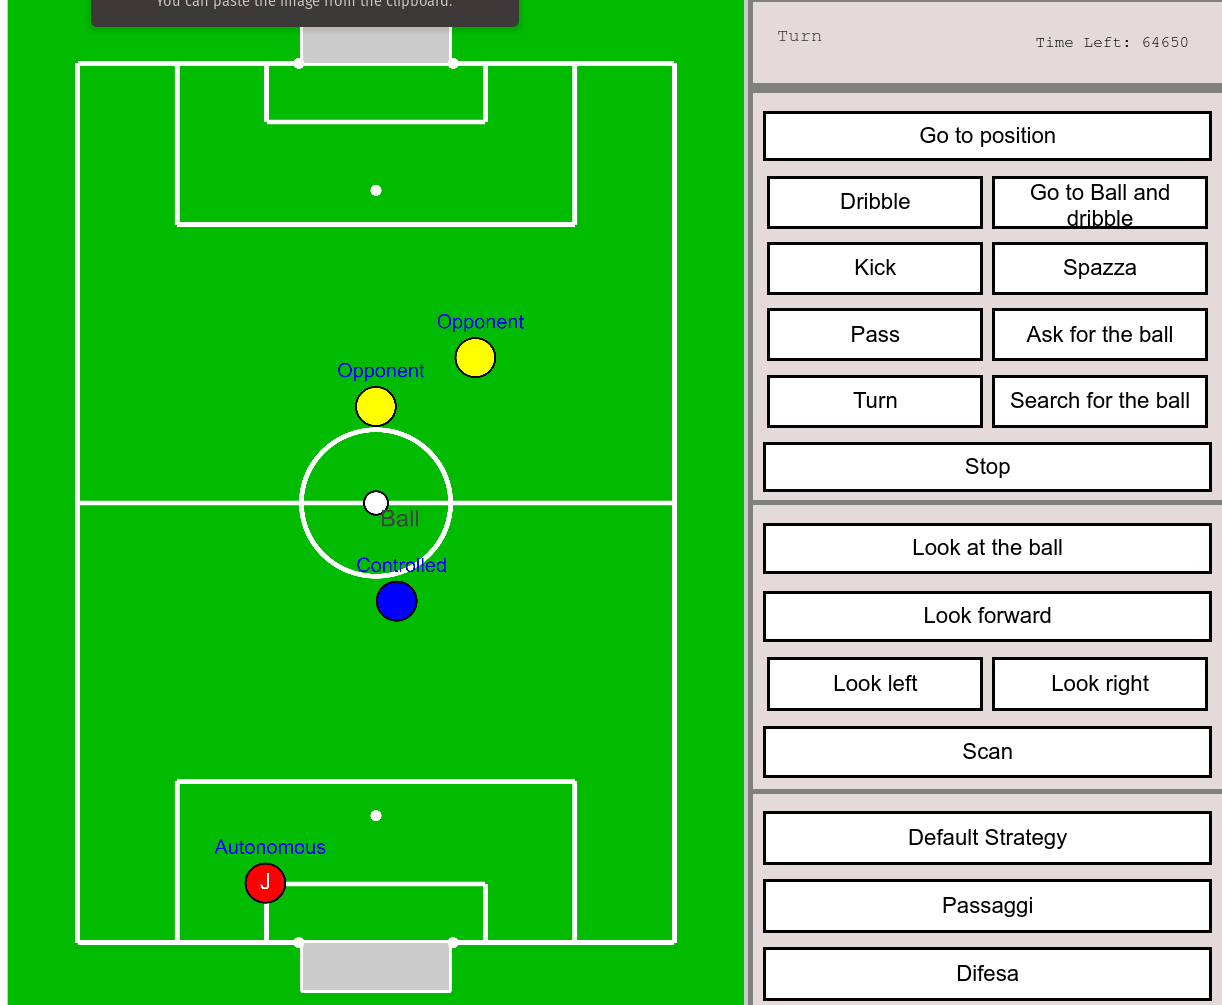
\includegraphics[width=0.9\linewidth]{assets/interface.png}
    \caption{The graphical interface}
    \label{fig:interface}
\end{figure}

\begin{figure}[H]
    \centering
    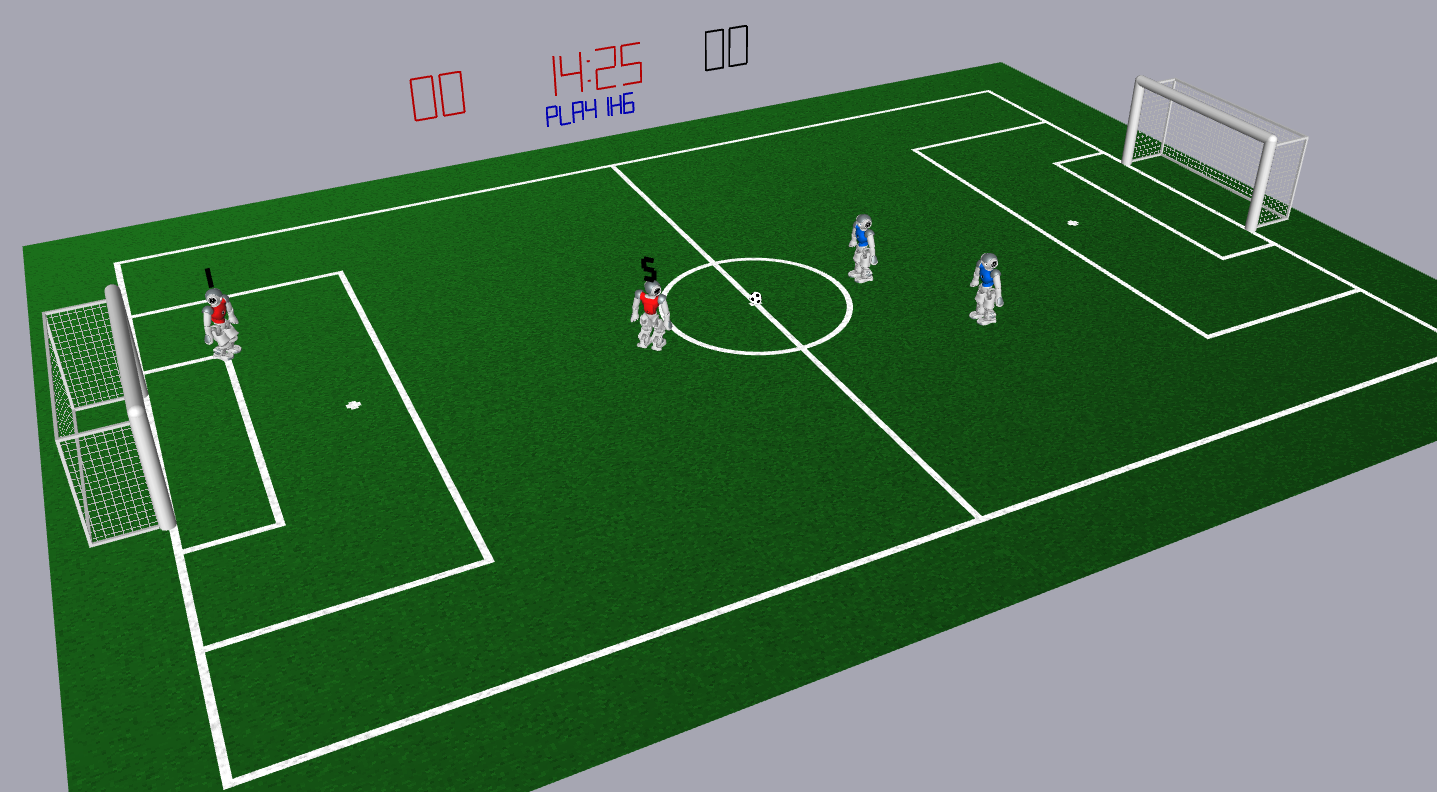
\includegraphics[width=0.9\linewidth]{assets/simrobot.png}
    \caption{The Corresponding Field Configuration}
    \label{fig:nao}
\end{figure}

\newpage
\section{Implementation}
\label{sec:impl}

From an implementative point of view, the system can be divided in four modules: 
\begin{itemize}
    \item \textbf{Communication Layer}: exchanges messages between the robot and the human operator
    \item \textbf{Framework}: the backbone of the system, which runs on the robot
    \item \textbf{GUI}: the graphical interface that allows the human operator to interact with the robot
    \item \textbf{Speech-to-Text Module}: the module that converts the human operator's voice commands to text
\end{itemize}

These modules are wrapped around the two main data structs that encapsulate the
exchanged messages, namely the \textit{HumanCommand} struct and the
\textit{DebugInfo} struct. The former is used to send commands from the human
operator to the robot. It has the following structure:
\begin{verbatim}
    1B: Command body
    1B: Command head
    1B: Strategy
    8B: [pos_x, pos_y]
    command_format: "<BBBff"
\end{verbatim}

Basically, it is formatted as a tuple of 5 elements, where the first three are
Bytes and the last two are floats. The last two elements are the coordinates of
the target position, which are indicated on the 2D field. This precise structure
is needed to be able to send the command through the socket and parse it on the
C++ side.

The \textit{DebugInfo} struct, on the other hand, is used to send feedback from
the robot to the human operator. It has the following structure:

\begin{verbatim}
1)      4B header
2)      1B version
3)      1B player_num
4)      1B team_num
5)      1B fallen
6-9)    3f (12B) [pos_x, pos_y, theta]
9)      1f (4B) ball_age
10-12)  2f (8B) [ball_pos_x, ball_pos_y]
12)     1H (2B) num_of_data_bytes
13)     1B player_role
14)     1B current_obs_size
15-35)  20B obstacle_types  
35-55)  20f (80B) obs_center_x
55-75)  20f (80B) obs_center_y
75-95)  20f (80B) obs_last_seen
95)     1H (2B) message_budget
96)     1H (2B) secs_remaining
97-99)  2B arm_contact
99-101) 2B arm_push_direction
101-103)2f (8B) arm_time_of_last_contact
103)    2f (8B) padding (whistle)
104-106) 2f (8B) teamball
106-108) 2f (8B) teamballvel
108)    12B padding

data_format: "<d4sBBBB3ff2fHBB20B20f20f20fHH2B2B2f2f2f2f12B"
\end{verbatim}

This data packet contains all the information that is needed to have a graphical
representation of the robot's mental model of the field.

The most important fields are:
\begin{itemize}
    \item \code{fallen}: a boolean that indicates if the robot is fallen,
    \item \code{pos\_x, pos\_y, theta}: the position of the robot in the field,
    \item \code{ball\_age}: the age of the ball that indicates how many cycles have passed since the robot saw the ball,
    \item \code{ball\_pos\_x, ball\_pos\_y}: the position of the ball in the field,
    \item \code{obstacle\_types}: an array that indicates the type of the obstacles in the field (e.g. teammate, opponent),
    \item \code{obs\_center\_x, obs\_center\_y}: the position of the obstacles in the field,
    \item \code{obs\_last\_seen}: the time when the obstacles were last seen,
    \item \code{secs\_remaining}: the time remaining in the game,
    \item \code{arm\_contact}: a boolean that indicates if the robot is in contact with an obstacle,
    \item \code{arm\_push\_direction}: the direction in which the robot arm is pushed,
    \item \code{arm\_time\_of\_last\_contact}: the time when the robot was last in contact with an obstacle,
    \item \code{teamball, teamballvel}: the position and velocity of the ball in the field.
\end{itemize}
Using these informations, the human operator can have a detailed view of the field through the robot's perceptions.

\subsection{Communication Layer}

The communication layer is responsible for the exchange of messages between the
robot and the human operator, in both directions. 
It is written in Python and based on UDP sockets. 

\subsubsection{Human-to-Robot communication}
The server listens to a port for a message from the graphical interface. Each unpacked message contains
the command in the form of a string, with any additional useful information for the execution of the instructions.
The receiving function from the GUI is the following:
\todo[inline]{cambia codice di receive}
\begin{verbatim}
def receive_command_from_js(self) -> tuple[int, int, int, int]:
    try:
        data, addr = self.server_socket.recvfrom(1024)
    except Exception as e:
        print(f"Error in receiving the message: {e}")
    try:
        message = data.decode()
    except UnicodeDecodeError:
        print(f"Received non-UTF-8 message from \
        JavaScript: {data} from {addr}")
    message_split = message.split('|')[1]
    content_message = message_split.split(',')
    task_type = content_message[2]
    command_number = Command[task_type].value
    strategy_number = int(content_message[5])
    task_label = content_message[4]
    selection = content_message[1]
    print(f"Task Label: {task_label}")
    if selection == "selection":
        x_position = int(content_message[6])
        y_position = int(content_message[7])
        print(f"X Position: {x_position}")
        print(f"Y Position: {y_position}")
    else:
        x_position = 0
        y_position = 0
    return command_number, strategy_number, x_position, y_position
\end{verbatim}

After the reception of the message, the whole instruction is wrapped in a serialized
struct and it is sent to the robot. All this is done through the following function:


\begin{verbatim}
def send_command_to_cpp(self, command: int, strategy: int, x: int, y: int):
    if command_number > self.config.command_offset:
        command_body_number = Command.Null.value
        command_head_number = command_number - self.config.command_offset
    else:
        command_body_number = command_number
        command_head_number = Command.Null.value
    encoded_data = struct.pack(
        self.config.command_format,
        command_body_number,
        command_head_number,
        strategy_number,
        x_position,
        y_position
    )
    try:
        client_socket.sendto(encoded_data, (robot_ip, command_send_port))
        print(f"Sending message to C++: {encoded_data}")
    except Exception as e:
        print(f"Error in send_message: {e}")
\end{verbatim}

\subsubsection{Robot-to-Human communication}
\todo[inline]{to check}
This thread makes the server listening to a different port for messages from the 
robot. As explained before, these messages contain world modeling data in
a packed way, and encorporate a lot of infos expressed above in the $DebugInfo$ struct.
The function that is responsible for receiving messages from the robot is the following:
\begin{verbatim}
    def receive_from_cpp(self) -> struct:
        debug_packet = None
        try:    
            data, _ = self.server_socket.recvfrom(1024)
        except Exception as e:
            print(f"Error in receiving the message: {e}")
        if len(data) == struct.calcsize(self.config.data_format):
            debug_packet = struct.unpack(self.config.data_format, data)
        else:
            print(f"Received unexpected data from C++: {data}")
        return debug_packet
\end{verbatim}

Then the server has to unwrap the debug packet and it is going to select just some of these information
to send to the graphcal interface. In particular, it will communicate the infos about the 
local mental model (see section \ref{subsec:mental_model}). It is done through these functions:

\begin{verbatim}
    def send_robot_pose(self, pos_x, pos_y, plot_id: int) -> None:
        robot_pose = f"{plot_id},{0.},{pos_x},{pos_y}"
        robot_pose_message = f"|robotPos:{robot_pose}"
        self.client_socket.sendto(robot_pose_message.encode(), \
            (self.config.local_ip, self.config.debug_send_port))
        
    def send_ball_info(self, debug_packet) -> None:
        ballpos_x = debug_packet[DataEntryIndex.BallPosX.value]
        ballpos_y = debug_packet[DataEntryIndex.BallPosY.value]
        ball_position = f"{ballpos_x:.2f},{ballpos_y:.2f}"
        ball_position_message = f"|ballPos:{ball_position}"
        self.client_socket.sendto(ball_position_message.encode(), \ 
            (self.config.local_ip, self.config.debug_send_port))
        
    def send_game_info(self, debug_packet) -> None:
        time_left = debug_packet[DataEntryIndex.SecsRemaining.value]
        time_left_message = f"|timeLeft:{time_left}"
        self.client_socket.sendto(time_left_message.encode(), \
            (self.config.local_ip, self.config.debug_send_port))

    def send_autonomous_role(self, debug_packet) -> None:
        current_me = self.debuginfo.controlled_robot.get_current()
        controlled_robot_pos_x = current_me[0]
        controlled_robot_pos_y = current_me[1]

        current_teammates = self.debuginfo.teammates.get_current()
        autonomous_robot_pos_x = current_teammates[0]
        autonomous_robot_pos_y = current_teammates[1]

        ball_pos_x = debug_packet[DataEntryIndex.BallPosX.value]
        ball_pos_y = debug_packet[DataEntryIndex.BallPosY.value]

        controlled_ball_distance = np.sqrt( \
            (controlled_robot_pos_x - ball_pos_x)**2 + \
            (controlled_robot_pos_y - ball_pos_y)**2)
        autonomous_ball_distance = np.sqrt( \
            (autonomous_robot_pos_x - ball_pos_x)**2 + \
            (autonomous_robot_pos_y - ball_pos_y)**2)

        autonomous_striker = \
            autonomous_ball_distance < controlled_ball_distance

        autonomous_info = f"|autonomousRole:{autonomous_striker}"
        self.client_socket.sendto(autonomous_info.encode(), \
            (self.config.local_ip, self.config.debug_send_port))
\end{verbatim}






\subsection{Framework}
\todo[inline]{to finish}
As it was previously said, the SPQR-Team framework is the backbone of the project and its
operational mechanism was explained in the section \ref{sec:framework}.
The two mental models are already available in the framework, which allow the robot to
maintain a representation of the world where he plays, \suggestion{permitting him to act according to
his needs, and helping us to give the right instructions to him.} 

What we added inside the framework (to make it work with the rest of the infrastructure) 
regard two aspects of the robot: the communication with the interface to send information
and receive human commands, and the behaviors the robot must have during the games, according
to own believes about the environment and to received human instructions.

\subsubsection{CommandReceiver and DebugMessageHandler}
The two main functions are the update of the CommandReceiver and the update of the DebugMessageHandler 
(which sends sensory information). The \textit{CommandReceiver} is responsible for updating the
representation \textit{HumanCommand} with the received command and additional parameters, 
while giving some audio feedback to the human about it. 
In the following function, the command is parsed,
converted to enums and stored in the provided representation. 

\begin{verbatim}
void CommandReceiver::update(HumanCommand& command) {
  
  if (theRobotInfo.number != RobotInfo::RoleNumber::controlled) return;
  
  char buffer[BUFFER_SIZE];
  int n = socket_read.read(buffer, BUFFER_SIZE);
  
  // First field (command_body): unsigned char
  HumanCommand::CommandBody received_command_body = 
      static_cast<HumanCommand::CommandBody>(buffer[0]);
  
  // Second field (command_head): unsigned char
  HumanCommand::CommandHead received_command_head = 
      static_cast<HumanCommand::CommandHead>(buffer[1]);
  
  // Third field (strategy): unsigned char
  HumanCommand::Strategy strategy = 
      static_cast<HumanCommand::Strategy>(buffer[2]);
  
  // Fourth field (x_pos): int (4 bytes)
  float x_pos;
  std::memcpy(&x_pos, buffer + 3, sizeof(x_pos));
  
  // Fifth field (y_pos): int (4 bytes)
  float y_pos;
  std::memcpy(&y_pos, buffer + 7, sizeof(y_pos));
  
  if (n > 0) {
      SystemCall::say(HumanCommand::CommandBody2String(received_command_body));
  
      if(received_command_body != HumanCommand::CommandBody::BaseCommandBody){
          command.commandBody = received_command_body;
          command.x = x_pos;
          command.y = y_pos;
      }
      if(received_command_head != HumanCommand::CommandHead::BaseCommandHead)
          command.commandHead = received_command_head;
  
      command.strategy = strategy;
  }
  return;
}
\end{verbatim}

The \textit{DebugMessageHandler} is responsible to update \dots
\todo[inline]{to complete, non so che scrivere}


\subsubsection{Designed behavior}
Once the command is received and the \textit{HumanCommand} representation is updated,
it is used by the specific behavior we designed for the interacting robot.
We created a \textit{BaseControlledCard} to convert the information inside the
representation in effective actions to execute. Due to the syntax of the CABSL standard
and to our necessities, we implemented the card to manage more clearly the body actions,
while implementing an auxiliar function (named \textit{switchHeadCommands}) to handle concurrently the head actions.
The body instructions are guided by a switch command, which directs the agent to the 
right state of the state-machine.
Here we show the root of the graph, whence all states branch off:

\begin{verbatim}
    initial_state(start)
    {
      transition
      {
        switch (theHumanCommand.commandBody)
        { 
        case HumanCommand::CommandBody::GoToPosition:
          goto goToPosition;
          break;
        case HumanCommand::CommandBody::Dribble:
          goto dribble;
          break;
        case HumanCommand::CommandBody::GoToBallAndDribble:
          goto goToBallAndDribble;
          break;
        case HumanCommand::CommandBody::Kick:
          goto kick;
          break;
        case HumanCommand::CommandBody::Spazza:
          goto spazza;
          break;
        case HumanCommand::CommandBody::Pass:
          goto pass;
          break;
        case HumanCommand::CommandBody::AskForTheBall:
          goto askForTheBall;
          break;
        case HumanCommand::CommandBody::Turn:
          goto turn;
          break;
        case HumanCommand::CommandBody::SearchTheBall:
          goto turn;
          break;
        case HumanCommand::CommandBody::Stop:
          goto stop;
          break;
        default:
          break;
        }
      }
    }
   
\end{verbatim}

It is possible to notice how each of these states correspond to a button in the interface,
as shown in the figure \ref{fig:interface}.
As explained in the section \ref{subsec:interface}, some of these states refer to lower 
level actions, which require the explicitation of the additional parameters by the human.
An example is the state \textit{goToPosition}:

\begin{verbatim}
    state(goToPosition)
    {
      transition
      {
        if (theHumanCommand.commandBody != HumanCommand::CommandBody::GoToPosition)
          goto start;
      }
      action
      {
        Pose2f pose = theLibMisc.glob2Rel(theHumanCommand.x, theHumanCommand.y);
        theWalkToPointSkill(pose);
        switchHeadCommands();
      }
    }

\end{verbatim}

which needs the field coordinates given by the operator (coach?) saved in the representation.
On the contrary, other actions must be interpreted just as \suggestion{ADVICE} coming 
from the coach. Here the agent has a certain degree of freedom, and must use 
its knowledge to complete the action. An example is the state \textit{goToBallAndDribble}:

\begin{verbatim}
    state(goToBallAndDribble)
    {
      transition
      {
        if (theHumanCommand.commandBody != HumanCommand::CommandBody::GoToBallAndDribble)
          goto start;
      }

      action
      {
        theGoToBallAndDribbleSkill(calcAngleToTarget(theLibStriker.strikerMovementPoint()));
      }
    }
\end{verbatim}
The called skill compute a free point in the field toward which the dribble must be executed,  
brings the robot near the ball and complete the dribble.
A special mention goes to the state \textit{pass}, which falls in the latter category of states.
This one tells to the agent to execute a passage to its teammate in the field, thus the robot
must have the position of the teammate in one of its mental model. 
At the time when the robot has no teammate, an uncertain situation appears.
We managed this circumstance redirecting to another action, applying a dribble instead of a passage.

\begin{verbatim}
state(pass)
{
    transition
    {
    if (theHumanCommand.commandBody != HumanCommand::CommandBody::Pass)
        goto start;
    }

    action
    {
    int num = theTeamData.numberOfActiveTeammates;
    int size = theTeamData.teammates.size();
    if(num > 0){
        theSaySkill("Pass the ball");
        Vector2f target = theTeamData.teammates[0].theRobotPose.translation;
        KickInfo::KickType kickType = theLibPass.getKickType(target);
        float distance = theLibMisc.distance(target, theRobotPose);
        theGoToBallAndKickSkill(calcAngleToTarget(target), 
            kickType, true, distance);
    }
    else{
        theSaySkill("Go to ball and dribble");
        theGoToBallAndDribbleSkill(calcAngleToTarget(
            theLibStriker.strikerMovementPoint()));
    }
    }
}
\end{verbatim}



\subsection{Speech-to-Text Module}
As a complementary feature of the interface, we integrate a Speech-to-Text module to enable voice 
interaction with the robot. This integration enhances the communication between the coach and the robot, 
making interactions faster and more efficient. In a dynamic environment like soccer, quick information 
exchange is crucial, and voice commands streamline the process.

\subsection{Interface}


\section{Results}
\label{sec:res}
\subsection{Usability}  
The system was tested exclusively by team members, and the feedback was positive 
across various aspects:  
\begin{itemize}  
    \item \textbf{Reliability}: The system underwent extensive testing before the RoboCup 
    SPL challenge and was used during the competition without any significant issues. 
    Communication between the robot and the human operator remained stable, with the 
    robot accurately executing commands and providing the expected feedback.  
    \item \textbf{Validity}: The robot successfully interpreted the human operator's 
    commands and executed them in real-time. Additionally, it provided the operator with a comprehensive view of the field through its sensors and offered feedback on the execution of commands.  
    \item \textbf{Sensitivity}: The system is sensitive to network delays, which can 
    impact the real-time interaction between the robot and the human operator.  
\end{itemize}  

The graphical interface was designed to be user-friendly and intuitive, ensuring that 
the human operator can interact with the robot quickly, which is essential in the 
competitive RoboCup SPL challenge, where each match lasts only 3 minutes.  

\subsection{Adversarial Environment - RoboCup 2024 SPL Challenge}  
The system was tested in the highly competitive and adversarial setting of the RoboCup 
2024 SPL challenge. Several factors in this environment could impact the system’s 
performance, such as:  
\begin{itemize}  
    \item \textbf{Network Delays}: The system’s real-time interaction can be affected 
    by network delays, posing challenges to command execution.  
    \item \textbf{Game Rules}: The robot must be capable of interpreting and adhering 
    to game rules in real-time.  
    \item \textbf{Opponent's Strategy}: Opponents aim to exploit any weaknesses in the 
    system, requiring the robot and the human-operator to adapt to their strategies dynamically.  
\end{itemize}  
Despite these challenges, the system performed effectively, and the team secured third 
place in the competition.  


\section{Experimental Evaluation} 

In this section we make some considerations about the efficacy of our pipeline by validating it experimentally. We focus on the Nao robot's performance in the RoboCup SPL 2024 competition and its effectiveness as an assistive player guided by a human coach. The goal of the evaluation is to assess how well the robot responds to both autonomous decision-making and human-provided instructions, and how these interactions impact its overall gameplay and decision-making quality during the tournament.

The primary research questions are:

\begin{enumerate}
    \item How accurately does the robot convey its mental model to the human operator?
    \item To what extent does the combination of autonomous behavior and human coaching enhance the robot’s performance in the competitive environment of RoboCup?
    \item How effectively does the human-robot interaction framework support timely and efficient communication under the constraints of real-time soccer gameplay?
\end{enumerate}

We have formulated the following hypotheses to address these questions. Firstly, we hypothesize that the robot is able to summarize well enough its perceptions by sending them to the 2D interface. We also hypothesize that the robot can correctly interpret and execute human commands in over 90\% of the given situations during the game. Thirdly, we hypothesize that the collaborative control system will enhance the robot's overall performance, leading to more effective gameplay and strategy adaptation compared to fully autonomous play. Lastly, we hypothesize that the communication framework will facilitate smooth, real-time interaction between the human coach and the robot, enabling responsive and coordinated action during the game.

\subsection{Experimental Variables}

To test these hypotheses, we have defined several key variables. The independent variables include:

\begin{itemize}
    \item \textbf{Control mode:} whether the robot operates autonomously or under human-assisted control.
    \item \textbf{Type of tactical scenario:} predictable (routine situations) vs. unpredictable (dynamic, novel situations).
    \item \textbf{Prior knowledge of the human coach:} whether the coach has a background in football (experienced) or no prior football coaching experience (inexperienced).
\end{itemize}

The dependent variables include:

\begin{itemize}
    \item \textbf{Decision-making accuracy:} measured by the robot's ability to correctly interpret and act on human commands in real-time.
    \item \textbf{Tactical performance:} measured by the robot's ability to adapt its strategy based on human input, especially in response to changing game conditions.
    \item \textbf{Overall game performance:} measured by key metrics such as goals scored, positioning, and game results.
\end{itemize}

By evaluating these variables, we aim to understand how the integration of human coaching impacts the robot’s performance in a competitive, high-pressure environment like RoboCup.

\subsection{Outcome}

By testing the pipeline directly in the RC24 Challenge we gained the following insights:
\begin{itemize}
    \item Given the commands are light-weight, they proved to be very effective and efficient, obtaining high accuracy and winning over other teams' more sophisticated approaches like using a portable console as interface, or also a visore. Also, the voice commands are especially useful in emergency situations , like the robot walking out of the field, where the GUI may be not the ideal choice. 
    \item The second and third indicator are somehow intertwined, since the second influences the third. We noticed that we were able to seamlessly integrate the human coached robot as if it were an automomous one on steroids. We were able to complete passages and score goals in a very reduced timespan, demonstrating once more how important the high-level decision-making layer is in the context of RoboCup.
\end{itemize}

The first and third independent variables are, of course, important factors to be considered in designing such a system and are somehow related. The most important question is how much autonomy to leave to the robot, since less knowledge of the human would require more autonomy by the robot. Our choice of leaving some degree of autonomy to the robot just for low level actions and world-modeling proved itself successful.

\section{Conclusion}
\label{sec:con}

In this project, we developed a system that enables real-time human-robot interaction in competitive soccer games, specifically targeting the RoboCup SPL 2024 challenge. By allowing a human operator to interact with a Nao humanoid robot through both voice commands and a graphical interface, the system demonstrated the potential for enhancing robotic performance in dynamic, real-world environments. The bidirectional communication framework, combined with the robot's mental modeling and real-time feedback capabilities, enabled the operator to act as a coach, offering strategic insights that improved the robot's decision-making on the field.

The success of our system in the RoboCup 2024 SPL challenge, where our team reached third place, validates the effectiveness of integrating human input into autonomous robot systems in high-pressure, time-sensitive scenarios. The project also highlights the importance of balancing local and global world models in collaborative robotics, ensuring accurate perception and effective execution of commands.

Future work could expand on this system by further refining the interaction between the robot and human, improving the robot's ability to interpret and prioritize human input in more complex scenarios and also with different modalities (e.g. gestures). Related to the latter, integrating more advanced social reasoning and context-aware behaviors could enhance the robot's autonomy, allowing for seamless transitions between human-provided instructions and self-driven actions.

Ultimately, this project represents a step forward in developing robust frameworks for human-robot collaboration in competitive environments, with potential applications extending beyond soccer games into broader fields where real-time human-robot communication is essential.


\bibliographystyle{unsrt}
\bibliography{references}

\end{document}
